\documentclass{standalone}

\usepackage{tikz}

\usepackage{pgfplots}
\pgfplotsset{compat=1.16}

\begin{document}
\centering
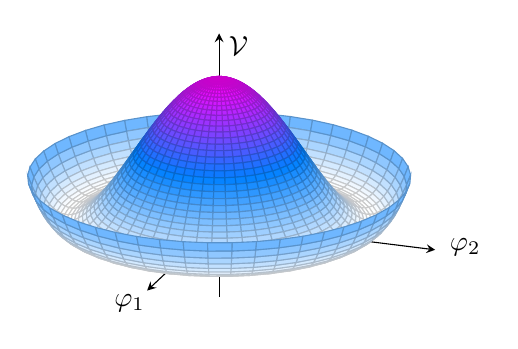
\begin{tikzpicture}
    \begin{axis}[
        % Gives axis instead of surronding box
        axis lines=center,
        view={110}{20},
        axis equal,
        samples=50,
        domain=0:360,       % Angle
        y domain=0:1.25,    % Radius
        ymax = 1.5, zmin=0, zmax=0.8,
        % Setting labels
        xlabel=$\varphi_1$,
        x label style={at={(0.296,0.1)}},
        ylabel=$\varphi_2$,
        y label style={at={(0.95,0.27)}},
        zlabel=$\mathcal{V}$,
        ticks=none,
        colormap/cool
    ]
    \addplot3 [
        surf,
        z buffer=sort,
        ] ({sin(x)*y}, {cos(x)*y}, {(y^2-1)^2});
  \end{axis}
\end{tikzpicture}
\end{document}
